\documentclass[../sparc.tex]{subfiles}
\graphicspath{{\subfix{../images/}}}
\begin{document}

%%%%%%%%%%%%%%%%%%%%%%%%%%%%%%%%%%%%%%%%%%%%%%%%%%%%%%%%%%%%%%%%%%%%%%%%%%%%%%%%
\section{Симулятор Wokwi}
Для того, чтобы программировать Arduino, не обязательно иметь реальную плату
Arduino -- вместо этого можно воспользоваться \emph{симулятором}.  Задача
симулятора -- программно эмулировать реальную плату с минимальными отличиями.

Вообще существуют два похожих термина: \emph{симулятор} и \emph{эмулятор}.

Посмотрим на различия\cite{so:simulator-vs-emulator} между ними:
\begin{itemize}
\item Задачей \emph{эмулятора} является имитация внешнего наблюдаемого поведения
  системы.  Внутреннее состояние механизма эмуляции не обязано точно повторять
  внутренее состояние того, что эмулируется.
\item Задачей \emph{симулятора} является моделирование внутреннего состояния
  симулируемой системы.  Конечным результатом хорошей симуляции является то, что
  виртуальная модель максимально близко повторяет целевую платформу.  В
  идеальном случае, вы должны иметь возможность посмотреть внутрь симуляции и
  обнаружить все аспекты работы, которые вы могли бы увидеть, посмотрев внутрь
  симулируемого объекта.
\end{itemize}

Симуляторы можно условно разделить на три категории:
\begin{itemize}
\item \emph{Offline-симуляторы} -- представляют собой отдельную программу,
  которую можно скачать, установить и запустить на компьютере пользователя
\item \emph{Online-симуляторы} -- специальные сайты, которые позволяют эмулировать
  аппаратную платформу прямо в браузере пользователя (либо полностью скачивая
  весь необходимый код в браузер, либо же выполняя часть операций на сервере.)
\item \emph{Комбинированные симуляторы} -- представляют собой отдельную
  программу, которая однако требует доступа в Internet для работы.
\end{itemize}

Online-эмуляторы проще в работе для начинающих пользователей, так как не требуют
установки чего-бы то ни было на компьютер.  Однако многие подобные эмуляторы
требуют регистрации, что не всем людям подходит.

Одним из свободно доступных online-эмуляторов, который не требует регистрации,
является проект Wokwi (\href{https://wokwi.com/}{wokwi.com}.)  Данный эмулятор
позволяет работать не только с платформами Arduino, но и с другими
микроконтроллерными платформами (вроде STM32 и ESP), а также с одноплатными
компьютерами.

Wokwi позволяет достаточно легко собирать проекты на базе Arduino,
программировать их и запускать.

Одним из ключевых параметров эмулятора является скорость работы -- чем быстрее
работает эмулятор, тем ближе к эмулируемой аппаратной платформе будет скорость
работы запускаемых проектов.  На скорость работы online-эмулятора Wokwi влияет
производительность вашего компьютера, вид браузера и сложность собранной схемы.

Самым оптимальным браузером для работы с Wokwi можно назвать Google Chrome или
же Chromium, однако Mozilla Firefox тоже неплохо справляется с задачей.

Wokwi имеет встроенную документацию по различным электронным компонентам,
которые можно использовать в схемах.

К недостаткам Wokwi, присутствующим на момент написания данного раздела, можно
отнести непостоянность скорости работы, что негативно влияет на эмуляцию схем,
требующих предсказуемого отклика (например, схемы, где идёт воспроизведение
звука.)  Другим недостатком для русскоговорящих пользователей является
англоязычность интерфейса, однако в современном мире широко доступных
переводчиков и распространения английского языка данный недостаток по нашему
мнению не является критическим.  Обратите внимание, что не рекомендуется делать
автоматический перевод страницы с редактором схем и кода, так как это может
нарушить работу эмулятора.

%%%%%%%%%%%%%%%%%%%%%%%%%%%%%%%%%%%%%%%%%%%%%%%%%%%%%%%%%%%%%%%%%%%%%%%%%%%%%%%%
\subsection{Начало работы}

Для того, чтобы начать работать с Arduino, на главной странице сайта Wokwi
небходимо в разделе ``Simulate with Wokwi Online'' (``Симулируйте вместе с Wokwi
Online'') выбрать вариант ``Arduino (Uno, Mega, Nano)''.  Далее надо промотать
страницу к разделу ``Start from Scratch'' (``Начать с нуля'') и выбрать там
желаемый вариант Arduino.

После этого откроется страница, где в левой части будет редактор кода (наподобие
Arduino IDE), а в правой части -- область сборки схемы.  Зелёная кнопка со
значком ``>'' в верхнем левом углу области сборки схемы позволяет запустить
проект в симуляторе.  Кнопка ``+'' позволяет выбрать и добавить компонент в
схему, а кнопка с тремя точками позволяет получить доступ к опциям симулятора.

%%%%%%%%%%%%%%%%%%%%%%%%%%%%%%%%%%%%%%%%%%%%%%%%%%%%%%%%%%%%%%%%%%%%%%%%%%%%%%%%
\newpage
\subsection{Компоненты для сборки схем}

\begin{longtable}{|>{
      \centering\arraybackslash
    }p{3cm}|>{
      \centering\arraybackslash}p{8cm}|
  }
\hline
Изображение & Описание \\ \hline
\endfirsthead

\hline
Изображение & Описание \\ \hline
\endhead

\hline
\parbox[t][1.4cm][c]{2cm}{\centering \vspace{1cm}
  
\includegraphics[width=0.12\textwidth]{wokwi/wokwi-led.png}} &
\parbox[t][3cm][t]{8cm}{\centering \textbf{Светодиод}\\ \raggedright

  Светодиод имеет два контакта: длинная ножка (``+'', анод), которая
  подключается к выходу Arduino через резистор, и короткая ножка (``-'', катод),
  которая подключается к GND (земле.)  Резистор необходим, так как без него
  светодиод может перегреться и выйти из строя, как и сама плата Arduino.

} \\  \hline

\parbox[t][0,5cm][c]{2cm}{\centering \vspace{1cm}
  
\includegraphics[width=0.12\textwidth]{wokwi/wokwi-resistor.png}} &
\parbox[t][2.6cm][t]{8cm}{\centering \textbf{Резистор}\\ \raggedright

  Резистор -- компонент, который ограничивает ток в электрической цепи и защищает
  другие компоненты от перегрузки.  Он применяется для регулировки тока, снижения
  напряжения и предотвращения повреждения компонентов.

} \\  \hline

\parbox[t][2,3cm][c]{2cm}{\centering \vspace{0.8cm}
  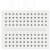
\includegraphics[width=0.12\textwidth]{wokwi/wokwi-breadboard.png}} &
\parbox[t][3.9cm][t]{8cm}{\centering \textbf{Макетная плата}\\ \raggedright

  Макетная плата -- это инструмент, который позволяет быстро и удобно создавать
  электрические цепи, не используя пайку.  Она состоит из ряда отверстий,
  соединенных проводящими дорожками.

} \\  \hline

\parbox[t][3,6cm][c]{2cm}{\centering \vspace{1cm}
  
\includegraphics[width=0.12\textwidth]{wokwi/wokwi-rgb-led.png}} &
\parbox[t][5.1cm][t]{8cm}{\centering \textbf{RGB-светодиод}\\ \raggedright

  RGB-светодиод -- это по сути три цветных светодиода, упакованных в один корпус:
  красный (англ. red), зеленый (англ. green) и синий (англ. blue.)  Эти цвета
  можно комбинировать между собой, для получения различных оттенков.  У
  RGB-светодиода обычно 4 контакта: один для общего анода (``+'') или катода
  (``-''), и по одному для каждого цвета.  Каждый из цветных контактов
  подключается к соответствующему пину на Arduino через резистор для ограничения
  тока, как обычный светодиод.

} \\  \hline

\parbox[t][2,8cm][c]{2cm}{\centering \vspace{1cm}
  
\includegraphics[width=0.12\textwidth]{wokwi/wokwi-lcd2004.png}} &
\parbox[t][4.3cm][t]{8cm}{\centering \textbf{Текстовый ЖК-дисплей}\\ \raggedright

  Текстовый ЖК-дисплей (LCD) -- это экран, который позволяет нам выводить
  текстовую информацию, использую жидкокристаллические элементы.  Он состоит из
  множества пикселей, котоыре могут быть включены для формирования символов.
  Для подключения дисплея к Arduino используется несколько пинов: пины для
  передачи данных (SDA и SCL) и питания (VCC (5V) и GND.)

} \\  \hline

\parbox[t][2,5cm][c]{2cm}{\centering \vspace{1cm}
  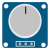
\includegraphics[width=0.12\textwidth]{wokwi/wokwi-potentiometer.png}} &
\parbox[t][4.3cm][t]{8cm}{\centering \textbf{Потенциометр}\\ \raggedright

  Потенциометр -- это регулируемый резистор, который позволяет изменять
  сопротивление в цепи, что, в свою очередь, позволяет контролировать различные
  параметры нашей системы (яркость, громкость, скорость и т.д.)  Обчыно имеет
  три контакта: два для подключения питания и земли, и средний контакт
  подключения к аналоговому входу на Arduino.  Вращением ручки изменяется
  положение подвижного контакта, что изменяет сопротивление между средним
  выводом и двумя остальными.

} \\  \hline

\parbox[t][1,8cm][c]{2cm}{\centering \vspace{1cm}
  
\includegraphics[width=0.12\textwidth]{wokwi/wokwi-buzzer.png}} &
\parbox[t][3.6cm][t]{8cm}{\centering \textbf{Зуммер}\\ \raggedright

  Зуммер (или динамик) -- это компонент, который позволяет нам выводить звук, при
  подаче на него электрического сигнала.  Имеет два контакта: анод (``+'',
  длинный контакт) длинный контакт, подключается к выходному пину Arduino и
  катод (``-'', короткий контакт), подключается к GND.

} \\  \hline

\caption{Некоторые компоненты, доступные в симуляторе Wokwi.}
\end{longtable}

\end{document}
